\PassOptionsToPackage{svgnames,dvipsnames,svgnames}{xcolor}

\documentclass[nonacm]{acmart}
\settopmatter{printfolios=true,printccs=false,printacmref=false}

%% Conference information
%% Supplied to authors by publisher for camera-ready submission;
%% use defaults for review submission.
%% ?

%% Copyright information
%% Supplied to authors (based on authors' rights management selection;
%% see authors.acm.org) by publisher for camera-ready submission;
%% use 'none' for review submission.
\setcopyright{none}
%\setcopyright{acmcopyright}
%\setcopyright{acmlicensed}
%\setcopyright{rightsretained}
%\copyrightyear{2019}           %% If different from \acmYear

%% Bibliography style
\bibliographystyle{ACM-Reference-Format}
%% Citation style
%\citestyle{acmauthoryear}  %% For author/year citations
%\citestyle{acmnumeric}     %% For numeric citations
%\setcitestyle{nosort}      %% With 'acmnumeric', to disable automatic
                            %% sorting of references within a single citation;
                            %% e.g., \cite{Smith99,Carpenter05,Baker12}
                            %% rendered as [14,5,2] rather than [2,5,14].
%\setcitesyle{nocompress}   %% With 'acmnumeric', to disable automatic
                            %% compression of sequential references within a
                            %% single citation;
                            %% e.g., \cite{Baker12,Baker14,Baker16}
                            %% rendered as [2,3,4] rather than [2-4].


%% Some recommended packages.
\usepackage{booktabs}   %% For formal tables:
                        %% http://ctan.org/pkg/booktabs
\usepackage{subcaption} %% For complex figures with subfigures/subcaptions
                        %% http://ctan.org/pkg/subcaption

\usepackage{microtype}
\usepackage{mdframed}
\usepackage{colortab}
\usepackage{mathpartir}
\usepackage{enumitem}
\usepackage{bbm}
\usepackage{stmaryrd}
\usepackage{mathtools}
\usepackage{leftidx}
\usepackage{todonotes}
\usepackage{xspace}
\usepackage{wrapfig}
\usepackage{float}

\usepackage{listings}%
\lstloadlanguages{ML}
\lstset{tabsize=2, 
basicstyle=\footnotesize\ttfamily, 
% keywordstyle=\sffamily,
commentstyle=\itshape\ttfamily\color{gray}, 
stringstyle=\ttfamily\color{purple},
mathescape=false,escapechar=\#,
numbers=left, numberstyle=\scriptsize\color{gray}\ttfamily, language=ML, showspaces=false,showstringspaces=false,xleftmargin=10pt, 
morekeywords={string, float, int},
classoffset=0,belowskip=\smallskipamount, aboveskip=\smallskipamount,
moredelim=**[is][\color{red}]{SSTR}{ESTR}
}

%% Joshua Dunfield macros
\def\OPTIONConf{1}%
\usepackage{joshuadunfield}

%% Can remove this eventually
\usepackage{blindtext}

\usepackage{enumitem}

% \newtheorem{theorem}{Theorem}[chapter]
% \newtheorem{lemma}[theorem]{Lemma}
% \newtheorem{corollary}[theorem]{Corollary}
% \newtheorem{definition}[theorem]{Definition}
% \newtheorem{assumption}[theorem]{Assumption}
% \newtheorem{condition}[theorem]{Condition}

\newtheoremstyle{slplain}% name
  {.15\baselineskip\@plus.1\baselineskip\@minus.1\baselineskip}% Space above
  {.15\baselineskip\@plus.1\baselineskip\@minus.1\baselineskip}% Space below
  {\slshape}% Body font
  {\parindent}%Indent amount (empty = no indent, \parindent = para indent)
  {\bfseries}%  Thm head font
  {.}%       Punctuation after thm head
  { }%      Space after thm head: " " = normal interword space;
        %       \newline = linebreak
  {}%       Thm head spec
\theoremstyle{slplain}
\newtheorem{thm}{Theorem}  % Numbered with the equation counter
\numberwithin{thm}{section}
\newtheorem{defn}[thm]{Definition}
\newtheorem{lem}[thm]{Lemma}
\newtheorem{prop}[thm]{Proposition}
% \newtheorem{cor}[section]{Corollary}     
% \newtheorem{lem}[section]{Lemma}         
% \newtheorem{prop}[section]{Proposition}  

% \setlength{\abovedisplayskip}{0pt}
% \setlength{\belowdisplayskip}{0pt}
% \setlength{\abovedisplayshortskip}{0pt}
% \setlength{\belowdisplayshortskip}{0pt}

\fancyfoot{} % suppresses the footer (also need \thispagestyle{empty} after \maketitle below)

% !TEX root = main.tex

\newcommand{\mynote}[3]{\textcolor{#3}{\textsf{{#2}}}}
\newcommand{\rkc}[1]{\mynote{rkc}{#1}{blue}}
\newcommand{\nick}[1]{\mynote{cy}{#1}{purple}}

\newcommand{\cvert}{{\,{\vert}\,}}

%% https://tex.stackexchange.com/questions/9796/how-to-add-todo-notes
\newcommand{\rkcTodo}[1]{\todo[linecolor=blue,backgroundcolor=blue!25,bordercolor=blue]{#1}}

\newcommand{\mattTodo}[1]{\todo[linecolor=green,backgroundcolor=green!2,bordercolor=green]{\tiny\textit{#1}}}
\newcommand{\mattOmit}[1]{\colorbox{yellow}{(Matt omitted stuff here)}}

\def\parahead#1{\paragraph{\textbf{#1.}}}
%% \def\paraheadNoDot#1{\paragraph{{\textbf{#1}}}}
\def\subparahead#1{\paragraph{\textit{#1.}}}
%% \def\paraheadindent#1{\paragraph{}\textit{#1.}}
%% \def\paraheadindentnodot#1{\paragraph{}\textit{#1}}

\newcommand{\ie}{i.e.}
\newcommand{\eg}{e.g.}
% \newcommand{\etc}{{\emph{etc.}}}
% \newcommand{\cf}{{\emph{cf.}}}
% \newcommand{\etal}{{\emph{et al.}}}

%% \newcommand{\hazel}{\ensuremath{\textsc{Hazel}}}
%% \newcommand{\sns}{\ensuremath{\textsc{Sketch-n-Sketch}}}
%% \newcommand{\deuce}{\ensuremath{\textsc{Deuce}}}
\newcommand{\Elm}{\ensuremath{\textsf{Elm}}}
\newcommand{\sns}{\ensuremath{\textrm{Sketch-n-Sketch}}}
\newcommand{\deuce}{\ensuremath{\textrm{Deuce}}}

\newcommand{\sectionDescription}[1]{\section{#1}}
\newcommand{\subsectionDescription}[1]{\subsection{#1}}
\newcommand{\subsubsectionDescription}[1]{\subsubsection{#1}}
%% \newcommand{\subsectionDescription}[1]{\subsection*{#1}}
\newcommand{\suppMaterials}{the Supplementary Materials}

\newcommand{\defeq}{\overset{\textrm{def}}{=}}

\newcommand{\eap}{action suggestion panel\xspace}
\newcommand{\Eap}{Action suggestion panel\xspace}

\newcommand{\myfootnote}[1]{\footnote{ #1}}

\def\sectionautorefname{Section}
\def\subsectionautorefname{Section}
\def\subsubsectionautorefname{Section}

\newcommand{\code}[1]{\lstinline{#1}}
\newcommand{\str}[1]
  {``#1''}

% Make italic?
%\newcommand{\Property}[1]{\emph{#1}}
\newcommand{\Property}[1]{\textrm{#1}}

% Calling out Cyrus's favorite verb, 'to be' ;)
\newcommand{\IS}{\colorbox{red}{is}\xspace}

\newcommand{\codeSize}
  %% {\footnotesize}
  {\small}

%\newcommand{\JoinTypes}[2]{\textsf{join}~~#1~~#2}
\newcommand{\JoinTypes}[2]{\textsf{join}(#1,#2)}

%% \newtheorem{theorem}{Theorem}[section] % 2.1, 2.2, etc.
\newtheorem{theorem}{Theorem}             % 1, 2, etc.
\newtheorem{remark}[theorem]{Remark}

%%%%%%%%%%%%%%%%%%%%%%%%%%%%%%%%%%%%%%%%%%%%%%%%%%%%%%%%%%%%%%%%%%%%%%%%%%%%%%%%
%% Spacing

\newcommand{\sep}{\hspace{0.06in}}
\newcommand{\sepPremise}{\hspace{0.20in}}
\newcommand{\hsepRule}{\hspace{0.20in}}
\newcommand{\vsepRuleHeight}{0.08in}
\newcommand{\vsepRule}{\vspace{\vsepRuleHeight}}
\newcommand{\miniSepOne}{\hspace{0.01in}}
\newcommand{\miniSepTwo}{\hspace{0.02in}}
\newcommand{\miniSepThree}{\hspace{0.03in}}
\newcommand{\miniSepFour}{\hspace{0.04in}}
\newcommand{\miniSepFive}{\hspace{0.05in}}
\newcommand{\breakAndIndent}
  {\mbox{}

   %% \hspace{0.15in}
   \hspace{0.00in}
  }

\newcommand{\justIndent}
  %% {\hspace{0.15in}
  {\hspace{0.00in}
  }

%%%%%%%%%%%%%%%%%%%%%%%%%%%%%%%%%%%%%%%%%%%%%%%%%%%%%%%%%%%%%%%%%%%%%%%%%%%%%%%%

% \lstset{
% %mathescape=true,basicstyle=\fontsize{8}{9}\ttfamily,
% literate={=>}{$\Rightarrow$}2
%          {<=}{$\leq$}2
%          {->}{${\rightarrow}$}1
%          {\\\\=}{\color{red}{$\lambda$}}2
%          {\\\\}{$\lambda$}2
%          {**}{$\times$}2
%          {*.}{${\color{blue}{\texttt{*.}}}$}2
%          {+.}{${\color{blue}{\texttt{+.}}}$}2
%          {<}{${\color{green}{\lhd}}$}1
%          {>?}{${\color{green}{\rhd}}$?}2
%          {<<}{${\color{green}{\blacktriangleleft}}$}1
%          {>>?}{${\color{green}{\blacktriangleright}}$?}2
%          {\{}{${\color{blue}{\{}}$}1
%          {\}}{${\color{blue}{\}}}$}1
%          {[}{${\color{purple}{[}}$}1
%          {]}{${\color{purple}{]}}$}1
%          {(}{${\color{darkgray}{\texttt{(}}}$}1
%          {)}{${\color{darkgray}{\texttt{)}}}$}1
%          {]]}{${\color{gray}{\big(}}$}1
%          {]]}{${\color{gray}{\big)}}$}1
% }

%%%%%%%%%%%%%%%%%%%%%%%%%%%%%%%%%%%%%%%%%%%%%%%%%%%%%%%%%%%%%%%%%%%%%%%%%%%%%%%%

\newcommand{\li}[1]{\lstinline[basicstyle=\ttfamily\fontsize{9pt}{1em}\selectfont]{#1}}
\newcommand{\lismall}[1]{\lstinline[basicstyle=\ttfamily\fontsize{9pt}{1em}\selectfont]{#1}}
\newcommand{\mapP}{\{0 \rightarrow \text{"a"}, 1 \rightarrow \text{"b"}, 3 \rightarrow \text{"c"}, 6 \rightarrow \text{"d"}, 10 \rightarrow \text{"e"}\}}
\newcommand{\dictP}{[(0, "a"), (0, "b"), (1, "c"), (2, "d"), (3, "e")]}

%%%%%%%%%%%%%%%%%%%%%%%%%%%%%%%%%%%%%%%%%%%%%%%%%%%%%%%%%%%%%%%%%%%%%%%%%%%%%%%%

%% \newcommand{\sal}{simple association list}
\newcommand{\sal}{association list}
\newcommand{\Sal}{Association List}

%% \newcommand{\cal}{canonicalized association list}
\newcommand{\cal}{canonical association list}
\newcommand{\Cal}{Canonical Association List}
\newcommand{\Cals}{Canonical association lists}

%% \newcommand{\fpf}{finite partial function}
\newcommand{\fpf}{partial function}
\newcommand{\Fpf}{Partial Function}
\newcommand{\Fpfs}{Partial functions}

\newcommand{\dd}{delta dictionary}
\newcommand{\dds}{delta dictionaries}
\newcommand{\Dd}{Delta Dictionary}
\newcommand{\Ddls}{Delta dictionaries}

%%%%%%%%%%%%%%%%%%%%%%%%%%%%%%%%%%%%%%%%%%%%%%%%%%%%%%%%%%%%%%%%%%%%%%%%%%%%%%%%

\newcommand{\SemTot}{Semantic Totality}
%% \newcommand{\SemInj}{Semantic Injectivity}
\newcommand{\SemInj}{Extensionality}
\newcommand{\EqDec}{Decidable Equality}
%% \newcommand{\EzDstr}{Ease of Destruction}
\newcommand{\EzDstr}{Easy Destructibility}

%% tweak and remove indirection macros later, once terminology settles
\newcommand{\Total}{\SemTot}
\newcommand{\Extensional}{\SemInj}
\newcommand{\DecidableEq}{\EqDec}
\newcommand{\Destructible}{\EzDstr}

\newcommand{\total}{Total}
\newcommand{\extensional}{Extensional}
\newcommand{\decidable}{Decid. Eq.}
\newcommand{\destructible}{Destructible}

\newcommand{\semanticallyTotal}{Semantically Total}
\newcommand{\destructed}{Destructed}

%%%%%%%%%%%%%%%%%%%%%%%%%%%%%%%%%%%%%%%%%%%%%%%%%%%%%%%%%%%%%%%%%%%%%%%%%%%%%%%%

% for use in alltt
\newcommand{\altFAll}{\ensuremath{\forall}}
\newcommand{\altRArr}{\ensuremath{\rightarrow}}
\newcommand{\altRARR}{\ensuremath{\Rightarrow}}
\newcommand{\altVdash}{\ensuremath{\vdash}}
\newcommand{\altTimes}{\ensuremath{\times}}
\newcommand{\altAnd}{\ensuremath{\land}}
\newcommand{\altOr}{\ensuremath{\lor}}
\newcommand{\altNE}{\ensuremath{\ne}}
\newcommand{\altEmpty}{\ensuremath{\varnothing}}
\newcommand{\altIn}{\ensuremath{\in}}
\newcommand{\altNIn}{\ensuremath{\notin}}
\newcommand{\altSum}{\ensuremath{\sum}}
\newcommand{\altLAng}{\ensuremath{\langle}}
\newcommand{\altRAng}{\ensuremath{\rangle}}
\newcommand{\altLamb}{\ensuremath{\lambda}}
\newcommand{\altGam}{\ensuremath{\Gamma}}
\newcommand{\altCirc}{\ensuremath{\circ}}
\newcommand{\altCdot}{\ensuremath{\cdot}}
\newcommand{\altBot}{\ensuremath{\bot}}

%% \input{macros} %% git rm macros.txt if not used

%\setlength{\abovecaptionskip}{4pt plus 3pt minus 2pt} % Chosen fairly arbitrarily
%\setlength{\belowcaptionskip}{-4pt plus 3pt minus 2pt} % Chosen fairly arbitrarily


\begin{document}

%% Title information
\title{Delta Dictionaries, or how to Cater Data Structures to Proof Assistants}

%% Author information
%% Contents and number of authors suppressed with 'anonymous'.
%% Each author should be introduced by \author, followed by
%% \authornote (optional), \orcid (optional), \affiliation, and
%% \email.
%% An author may have multiple affiliations and/or emails; repeat the
%% appropriate command.
%% Many elements are not rendered, but should be provided for metadata
%% extraction tools.

% ACM member number: ?
% \author{?}
% \authornote{with author1 note}          %% \authornote is optional;
                                        %% can be repeated if necessary
% \orcid{nnnn-nnnn-nnnn-nnnn}             %% \orcid is optional
%\affiliation{
%  \position{Graduate student}
%  % \department{Department1}              %% \department is recommended
%  \institution{University of Chicago}            %% \institution is required
%  % \streetaddress{Street1 Address1}
%  % \city{City1}
%  % \state{State1}
%  % \postcode{Post-Code1}
%  % \country{Country1}
%}
%\email{nickmc@uchicago.edu}          %% \email is recommended

%% Paper note
%% The \thanks command may be used to create a "paper note" ---
%% similar to a title note or an author note, but not explicitly
%% associated with a particular element.  It will appear immediately
%% above the permission/copyright statement.
% \thanks{with paper note}                %% \thanks is optional
                                        %% can be repeated if necesary
                                        %% contents suppressed with 'anonymous'

TODO TODO TODO remaining info, e.g. ACM member number and author info or whatev

%% Abstract
%% Note: \begin{abstract}...\end{abstract} environment must come
%% before \maketitle command
% !TEX root = ?.tex

%% no citations in Abstract
%%
%% \cite{?}

\begin{abstract}

Dictionaries, or finite maps, are a core data structure in any programming language.
%
General-purpose languages implement dictionaries with hash tables or balanced trees, but proof assistants---which favor simplicity and provability over performance---generally employ association lists or finite partial functions.
%
Though suitable for many uses, each solution has drawbacks:
%
association lists allow arbitrary order and may contain duplicates (unless refined with an explicit proof about validity), and
%
partial functions cannot be compared for equality
%
nor easily destructed.

We develop a novel list-based representation, called \emph{delta dictionaries}, that simultaneously achieves benefits of the conventional representations.
%
Delta dictionaries are \emph{total} (every type-correct list is semantically valid),
%
\emph{extensional} (there is a one-to-one correspondence between lists and semantic mappings), and
%
\emph{destructible} (the internal representation can be inspected as needed).
%
We present the implementation of delta dictionaries and relevant metatheory---formalized in Agda---and we discuss when delta dictionaries may or may not be preferable to conventional solutions.

%% Using a variant of delta-encoding, we develop a novel list-based solution that preserves
%% canonical ordering while ensuring that every type-correct list is semantically valid, eliminating the need for refinement
%% with a proof of validity. Our solution also establishes a one-to-one correspondence between dictionary terms and semantic
%% mappings. We demonstrate the practical importance of these properties when developing metatheory for environment-based
%% evaluation semantics, while acknowledging that drawbacks of our solution may make it inferior to one of the conventional
%% solutions in some cases where that conventional solution is viable. We prove the relevant metatheory in Agda.

%
% Our solution is not suitable for all key types, and is harder to destruct or
%iterate than other list-of-pair solutions, but is nonetheless better suited to many large, complex program
%foundations metatheories than the existing solutions.
%
% Although easy to define and reason about, this approach has the disadvantage that keys
%can be duplicated, leading to the fact that many distinct lists represent the same semantic mapping.
%This many-one relationship creates various difficulties when used in practice, such as when proving
%contraction and exchange for a type-checking judgment.

\end{abstract}

\input{defs}

%% Keywords
%% comma separated list
% \keywords{keyword1, keyword2, keyword3}  %% \keywords is optional
% \keywords{..., ...}

%% \maketitle
%% Note: \maketitle command must come after title commands, author
%% commands, abstract environment, Computing Classification System
%% environment and commands, and keywords command.
\maketitle
\thispagestyle{empty} % suppresses the footer

\section{Introduction}
\label{sec:Introduction}

\newcommand{\firstUseGoal}[1]
  %% {\emph{#1}}
  %% {\textbf{#1}}
  {\textbf{\emph{#1}}}

%%%%%%%%%%%%%%%%%%%%%%%%%%%%%%%%%%%%%%%%%%%%%%%%%%%%%%%%%%%%%%%%%%%%%%%%%%%%%%%%
%% \rkc{Part 1.1: Motivation and SAL/CAL/FPF. Editing TBD.}

\subsection{Background}

This paper assumes familiarity with statically typed functional languages (\eg{} Haskell, OCaml), and relevant concepts such as Hindley-Milner type systems, pattern-matching, data types, and product types.
%
A cursory background on \emph{proof assistants} and \emph{dependent types} is developed during the course of this introduction, but unfamiliar readers are encouraged to review a more thorough treatment such as \citep{plfa} or \citep{Pierce:SF1}.

A \emph{proof assistant} is a programming language with first-class support for defining and proving theorems, together with editor tools that ease the development of proofs.
%
Many popular proof languages, including Coq and Agda, are founded on \emph{dependent types}, in which a type can be parameterized by concrete values such as numbers, lists, or functions,
%
and in which theorems are types, proofs are functions (or other concrete values), and type checking subsumes proof checking.

In most programming contexts, the design of data structures and algorithms is chiefly focused on performance, but in dependently-typed proof assistants, evaluation performance is often unimportant since checking a proof requires type-checking but not actual evaluation.
%
As such, proof assistants often use entirely different data structures than those of conventional settings, with a focus on simplicity or useful proof-theoretic properties.

This paper considers several approaches to implementing \emph{dictionaries}, \ie{} finite mappings from keys to values.
%
The dictionary is a fundamental utility in most programming contexts and serves a broad range of purposes, so the choice of implementation is very important.
%
In conventional languages, dictionaries are implemented with auto-balanced trees or hashtables, which are highly performant, but also very complicated.

\subsection{Conventional Solutions}

\parahead{\Sal{}s}

The simplest representation for a dictionary, an \emph{\sal}, is merely a list of key-value pairs~\citep[Lists]{Pierce:SF1}.
%
Insertion and destruction are trivially achieved by the cons operator and pattern matching, respectively.
%
Lookup is only slightly more involved:
%
\begin{alltt}
  -- assumes that the key type K is fixed
  -- \altFAll\{V\} is an implicit type parameter
  assoc-list-lookup : \altFAll\{V\} \altRArr List (K \altTimes V) \altRArr K \altRArr Maybe V
  assoc-list-lookup [] \_ = None
  assoc-list-lookup ((k1 , v1) :: l) k =
    -- eq-dec-K returns Inl if its args are equal, Inr otherwise
    with eq-dec-K k k1
  ... | Inl \_ = Some v1
  ... | Inr \_ = assoc-list-lookup l k
\end{alltt}

Though easy to work with and reason about, \sal{}s have a drawback which can cause difficulty during proof development:
%
because they allow duplicate bindings for the same key and they are sensitive to the order of insertions, many distinct \sal{}s represent the same semantic mapping.
%
For example, the first two lines of \autoref{fig:intro-example}
%
show two distinct association lists (among others) that represent a dictionary with three particular bindings.
%
This lack of \firstUseGoal{\Extensional} can make proofs more difficult~\cite[Maps]{Pierce:SF1} or impossible, especially when it comes to proving \emph{contraction} and \emph{exchange}~\citep{StructProp}
%
as discussed further in \autoref{sec:CaseStudy} and \autoref{sec:Discussion:Generality}.

%% \begin{figure}[b]
%% \begin{figure}[h]
  \centering
  \begin{tikzpicture}[nodes = {align = left}]
    %% \node [scale=.45]
    \node [scale=.33]
    {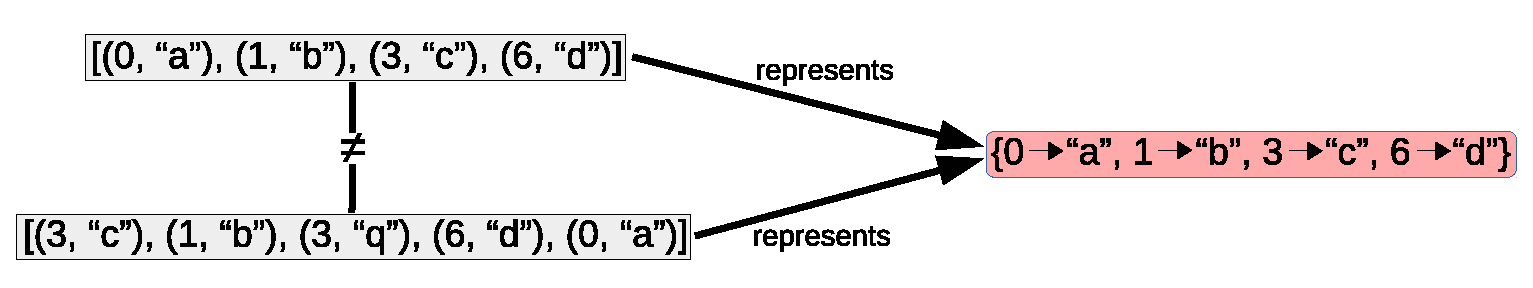
\includegraphics{figs/unequal.eps}};
  \end{tikzpicture}
  \caption{Two distinct \sal{}s representing the same semantic mapping. \rkc{Let's show the first two rows from Fig 1. And let's fit this into one column.}}
  \label{fig:uneq}
\end{figure}


\parahead{\Cals}

To establish a one-to-one correspondence between association lists and semantic mappings, one solution~\citep{FMapList} is to maintain a \emph{canonical}
%
form that is semantically valid and unique, namely, a list in which there are no duplicate keys and, furthermore, where keys are in sorted order.%
%
\footnote{\hspace{0.01in}%
%
The Coq standard library~\citep{FMapInterface}, describes unordered but deduplicated \sal{}s as ``weak,'' implying that \cal{}s are ``strong.''
%
}
%
The second association list shown in \autoref{fig:intro-example} is one such example.
%
This approach requires a more sophisticated \texttt{insert} function than that of the naive \sal{} approach:
\begin{alltt}
  -- assumes that the key type K is fixed
  cal-insert : \altFAll\{V\} \altRArr List (K \altTimes V) \altRArr (K \altTimes V) \altRArr List (K \altTimes V)
  cal-insert [] (k , v) = (k , v) :: []
  cal-insert ((k1 , v1) :: l) (k , v) =
    with ord-dec-K k k1
  ... | Inl \_       = (k , v) :: (k1 , v1) :: l         -- k < k1
  ... | Inr (Inl \_) = (k , v) :: l                      -- k == k1
  ... | Inr (Inr \_) = (k1 , v1) :: cal-insert l (k , v) -- k > k1
\end{alltt}

Despite being a bit more complicated, this approach has the benefit of being \extensional{}, in that if any two valid lists are not identical, they must have distinct semantic meanings.
%
The property of \SemInj{} is important for several reasons - in particular it permits the use of the built-in equality proposition to establish semantic equivalence.
%
Proof languages such as Agda have built-in support for \emph{reflexive equality}, which judges two values (of the same type) as being equal if and only if they are precisely identical:
\begin{alltt}
  -- In Agda, 'Set' is (roughly) the type of all types (incl. propositions).
  -- \_==\_ means that == is infix and binary.
  -- The first explicit arg is named x and is of type T,
  -- the second explicit arg is also of type T but is unnamed.
  -- Because == is a proposition, the "return type" is Set.
  data \_==\_ \{T : Set\} (x : T) : T \altRArr Set where
    -- A constructor of a proposition is a proof of that proposition.
    -- refl is the only constructor - for any x, refl is a proof that x == x.
    refl : x == x
    -- There's no way to establish equality of two arbitrary values x and y.
\end{alltt}

The built-in equality proposition is a common and intuitive way to judge the equality of two values.
%
Furthermore, proof assistants have special features for working with it, which can be harnessed to simlify and expedite proof development.
%
As such, it's very useful to be able to use this proposition, rather than to define a custom proposition that judges the semantic equivalence of two dictionaries.

Although the \cal{} approach is \extensional, it has another drawback; the list-of-pairs type allows arbitrary, possibly invalid lists, so each \cal{} must be packaged with a proof of validity:
\begin{alltt}
  -- assumes that the key type K is fixed
  data \_valid-cal \altFAll\{V\} (List (K \altTimes V)) : Set
    EmptyVal  : [] valid-cal
    SingleVal : \altFAll\{k v\} \altRArr ((k , v) :: []) valid-cal
    -- For any k1, k2, v1, v2, and l, if k1 < k2, and (k2 , v2) :: l is valid,
    -- then ManyVal stands as a proof that (k1 , v1) :: (k2 , v2) :: l is valid.
    ManyVal   : \altFAll\{k1 k2 v1 v2 l\} \altRArr
                  k1 < k2 \altRArr
                  ((k2 , v2) :: l) valid-cal \altRArr
                  ((k1 , v1) :: (k2 , v2) :: l) valid-cal

  cal : \altFAll\{V\} \altRArr Set
  -- '\altSum[ x \altIn T ] (p x)' packages x (of type T) with a proof that it satisfies p
  cal \{V\} = \altSum[ l \altIn List (K \altTimes V) ] (l valid-cal)
\end{alltt}

This paper coins the term \firstUseGoal{\semanticallyTotal} to describe any data structure whose type is free of proof terms and yet contains no invalid members -
%
\ie{} the mapping from values in the underlying type to their semantic meanings is total.
%
To illustrate, a pair of integers is not a \semanticallyTotal{} data structure for the rational numbers, since if the second integer is $0$ then the pair is invalid,
%
but a pair of an integer and a natural, where the natural represents the denominator minus $1$, \emph{is} \semanticallyTotal{} (note that neither of these data structures is \extensional).
%
The downsides of having to use validity proofs are discussed further in \autoref{sec:CaseStudy} and \autoref{sec:Discussion:Generality}.

\parahead{\Fpfs}

A third conventional solution is to represent dictionaries as finite partial functions~\cite[Maps]{Pierce:SF1} (\ie{} functions that return \texttt{None} for all but finitely many inputs).
%
The third line of \autoref{fig:intro-example} depicts a nested $\lambda$-expression that serves as the ``lookup table'' (we omit the \texttt{Some} constructors for space).
%
This approach can be made \extensional{} by postulating \emph{functional extensionality}~\mbox{\cite[Logic]{Pierce:SF1}}, which axiomatically asserts that $(\forall x, f(x) == g(x)) \Rightarrow f == g$.
%
On the other hand, this approach technically fails to satisfy \SemTot, since the function type permits \emph{non-}finite maps.
%
Even so, this is often not a problem in practice -- as long as the dictionary is never iterated, destructed, or counted, an infinite dictionary is indistinguishable from a finite dictionary.
%
Furthermore, a dictionary built from a finite program can only have finitely many mappings.
%
The more serious problem is that, unlike either association list approach, functions lack \firstUseGoal{\DecidableEq} and cannot be \firstUseGoal{\destructed}.

While a proof that $x == y$ establishes the truth that $x$ and $y$ are equal, the \texttt{==} proposition is not capable of \emph{deciding} whether or not two arbitrary values are equal.
%
To \emph{decide} this question, we need to define a function that accepts two arguments (of the same type) and returns either a proof that they are equal or a proof that they are not equal:
\begin{alltt}
  -- 'P \altRArr \altBot' means that P is false.
  eq-dec-K : (x y : K) \altRArr ((x == y) \altOr (x == y \altRArr \altBot))
  eq-dec-K x y = ?  --  the implementation will depend on the type K
\end{alltt}

Note that proof languages like Coq and Agda are \emph{constructive}; they elide the \emph{law of the excluded middle}, so it's possible for a proposition to be neither provably true nor provably false.
%
As such, the ability to decide whether some proposition (such as the equality of two values) is true or false cannot be taken for granted -- if this ability is needed, it must be explicitly established by defining a function such as the one above.
%
In the case of functions, it's not possible to establish that two arbitrary functions are unequal, so there is no way to establish decidability.
%
Naturally, deciding whether or not two dictionaries are equal is important and useful for many of the same reasons it would be in a more conventional language, so the lack of \DecidableEq{} is a substantial weakness.

The inability to destruct a function is more intuitive -- destruction is essentially the same as in other functional languages, where pattern-matching is typically used to separate one element of a collection (often the \emph{head}) from the rest of the collection.
%
A lambda value can't be destructed or picked apart in any way, so its values also can't be iterated or counted.
%
The function could be packaged with a set indicating its domain --- \ie{}~a canonical list of keys --- but would then have to include a proof that those keys are correct, violating \SemTot{} in the same troublesome way that \cal{}s do.

\subsection{Core Properties}

In some cases, the aforementioned drawbacks are minor or can be worked around.
%
But developing large proofs is challenging, so any stumbling block can cause exorbitant increases in verbosity, time, effort, and accidental complexity.
%
Furthermore, as shown in \autoref{sec:CaseStudy}, there are cases where these drawbacks make a proof task not merely difficult, but outright impossible.

%%%%%%%%%%%%%%%%%%%%%%%%%%%%%%%%%%%%%%%%%%%%%%%%%%%%%%%%%%%%%%%%%%%%%%%%%%%%%%%%
%% \rkc{Part 1.2: Summary of Design Goals. Editing TBD.}

Ideally, when working in a proof assistant, an implementation of a data structure---dictionaries in particular for this paper---would satisfy the following properties:

\newcommand{\designGoal}[1]
  {\textbf{\emph{#1:}}}

\begin{enumerate}

\item
%
\designGoal{\SemTot}
%
Every value in the representation type is semantically valid, \ie{}~the mapping from values to their semantic meanings is total.

\item
%
\designGoal{\SemInj}
%
Built-in equality corresponds to semantic equivalence, \ie{} two unequal values have different semantic meanings.

\item
%
\designGoal{\EqDec}
%
Built-in equality is decidable for the representation type.

\end{enumerate}

Furthermore, in addition to properties about the external interface of the data structure, it is often useful to retain the ability to inspect, iterate, and manipulate sub-dictionaries.
%
%% Thus, our final design goal:

\begin{enumerate}

\item[(4)]
%
\designGoal{\EzDstr}
%
The ability to decompose a data structure into atomic subparts in a convenient manner.

%% to facilitate

%% sufficiently

\end{enumerate}

\newcommand{\no}
  %% {No}
  {}
\newcommand{\yes}
  %% {Yes}
  %% {\phantom{*}\cmark\phantom{*}}
  {\phantom{$^-$}\cmark\phantom{$^-$}}
\newcommand{\yesBut}
  %% {Yes*}
  %% {\phantom{*}\cmark*}
  {\phantom{$^-$}\cmark$^-$}
\newcommand{\eq}
  %% {Decidable equality}
  {Eq K}
\newcommand{\ord}
  %% {Orderable}
  {Eq K, Ord K}
\newcommand{\isoNat}
  %% {Bijects to naturals}
  {K $\leftrightarrow$ Nat}
\newcommand{\verySimple}
  %% {+1}
  %% {\cmark\!\!\cmark}
  {\phantom{$^+$}\cmark$^+$}
\newcommand{\simple}
  %% {0}
  %% {\cmark}
  {\phantom{$^+$}\cmark\phantom{$^+$}}
\newcommand{\hard}
  %% {-1}
  {}

%% \begin{figure}[H]
\begin{figure*}
  \begin{tabular}{ l || c | c | c | c | c || c}
            & \multicolumn{5}{c||}{Client Usage}                             & Implementation
   \\ \hline
            & \total & \injective & \comparable & \destructible & Key Type K & Simple
   \\ \hline
   \Sal     & \yes   & \no        & \yes        & \yes          & \eq        & \verySimple
   \\ %% \hline
   \Cal     & \no    & \yes       & \yes        & \yes          & \ord       & \simple
   \\ %% \hline
   \Fpf     & \no(TODO)   & \yes  & \no         & \no           & \eq        & \verySimple
   \\ %% \hline
   \Cfpf    & ...    & ...        & ...         & ...           & \ord       & \simple
   \\ %% \hline
   \Dd      & \yes   & \yes       & \yes        & \yesBut       & \isoNat    & \hard
  \end{tabular}
  \caption{Properties of dictionary representations.}
  \label{fig:prop-summary}
\end{figure*}
%% \end{figure}


\autoref{fig:prop-summary} summarizes the preceding discussion along these dimensions; note that the association list representations can be easily destructed, but destruction is not possible for \fpf{}s.
%
None of the conventional approaches satisfies both \SemTot{} and \SemInj{}, nor more than three of the four properties.

\subsection{Novel Solution: Delta Dictionaries}
%
The four core properties can be (mostly) satisfied by way of \emph{\dds{}} -- although destructible, \EzDstr{} is not fully achieved because destruction of \dds{} is awkward.
%
%% A \dd{} is similar to a canonical association list, but instead of storing each literal key value, it stores the \emph{difference} from the previous key, minus 1.
%
A \dd{} can be described as a ``canonical-by-construction'' association list: instead of storing each literal key value, it stores the \emph{difference} from the previous key, minus 1 (details in \autoref{sec:DD}).
%
For example, compare the canonical association list and \dd{} in \autoref{fig:intro-example}:

\vsepRule

%% keep this in sync with Figure 1
\begin{tabular}{ l l }
 \Cal{} & [(1, \str{a}), (3, \str{b}), (6, \str{c})] \\
 \Dd{}  & [(1, \str{a}), (1, \str{b}), (2, \str{c})]
\end{tabular}

\vsepRule

Every well-typed list-of-pairs is a valid \dd{}, thus no proof term is needed to establish validity (\SemTot).
%
Every unique \dd{} represents a unique semantic mapping, thus built-in equality may be used for semantic equivalence (\SemInj).
%
%% there is a bijection between \dd{} terms and finite maps,
%
Furthermore, we define a function which determines whether or not two \dds{} are equal (\EqDec), and a \texttt{destruct} function, which permits destruction albeit in a more awkward manner than standard pattern matching.

As summarized in \autoref{fig:prop-summary}, delta dictionaries strike a new balance in this design space.
%
Compared to \cal{}s, \dds{} enjoy \SemTot{}---the lone property among those we identify which the \cal{} does not.
%
However, destruction and iteration for \dds{} is substantially more difficult.
%
Furthermore, unlike all of the conventional approaches, \dds{} require a bijection to the naturals, not merely decidable equality or ordering, for their key types.
%
%% Our definition and implementation uses natural numbers for keys, and we illustrate how to use bijections to the naturals as a way of supporting strings, integers, or other key types that can be bijected to the naturals without great difficulty.
%
Lastly, though not a concern from a client's perspective, the implementation of delta dictionaries is considerably more involved than the conventional approaches.

%% than it is with the {\SAL}s or {\CAL}s, for which these operations are trivial ({\FPF}s cannot be properly destructed at all).

%% Naturally, \dds~ have some drawbacks as well.

%% Although most types that are suitable for use as keys in the first place can be bijected to the
%% naturals, for some types defining this bijection may be too awkward or cumbersome, in which case \dds~ may
%% be a poor choice.

%% As with the drawbacks of the other solutions, this one is
%% discussed further in the \nameref{sec:Problem} section.

\subsection{Outline}
%
%% Next, we describe the core operations for delta dictionaries in \autoref{sec:DD} and the relevant metatheory in \autoref{sec:DD:props}.
%
Next, we describe the core operations for delta dictionaries and the relevant metatheory in \autoref{sec:DD}.
%
In \autoref{sec:CaseStudy}, we describe a small case study in proof development that demonstrates the necessity of delta dictionaries.
%
Finally, we conclude in \autoref{sec:Discussion} with a discussion. %% of related work.
%
%% Our implementation and proofs are formalized in Agda and available in the anonymous supplementary materials.


%% {\color{gray}
%% 
%% \subsection{\rkc{Grab Bag of Text}}
%% 
%% %% \section{Problem}
%% %% \subsection{Problem}
%% %% \label{sec:Problem}
%% 
%% \rkc{1}
%% 
%% Data structures can possess or lack a wide range of properties that make them easier or harder to work with
%% when proving metatheory. Naturally, when possible, data structures should be chosen that posess those
%% properties which make the task at hand easier. Achieving this requires identifying the valuable properties,
%% what it is that makes them valuable, and finding or inventing data structures which possess those properties.
%% We hold that this is a broad topic of
%% research, which we illustrate in the particular context of choosing an implementation for a dictionary. In
%% this context, we identify, according to both conceptual and practical considerations, four important and
%% discriminating properties that a dictionary implementation may or may not possess:
%% TODO there's a good chance some of these properties have been named somewhere else. We should make sure we
%% don't try and coin terms for anything that's already been defined somewhere.
%% 
%% % TODO we may decide that the conceptual and practical benefits of decidable equality are so obvious or
%% % self-evident that we don't need any further discussion of that property
%% 
%% %% \subsection{Conceptual Importance}
%% %% \label{sec:Problem:concept}
%% 
%% \rkc{2}
%% 
%% In \autoref{sec:Problem:pract}, we illustrate practical problems and benefits under the particular context
%% of choosing an implementation for dictionaries. But first, it's worth exploring conceptual aspects that
%% apply to the general case. These conceptual aspects capture the spirit of practical considerations and
%% motivate the search for solutions that are not merely serviceable but elegant, moral, and insightful.
%% 
%% \subsubsection{\SemTot}
%% \label{sec:Problem:concept:SemTot}
%% TODO something something "making impossible states impossible", i think allusion to the right parts out of that
%% video will suffice to make the point here
%% 
%% \subsubsection{\SemInj}
%% \label{sec:Problem:concept:SemInj}
%% TODO something something it yields arbitrariness, which is not always wrong but which is unaesthetic and, when
%% avoidable, undesirable. It also allows for a semantic meaning to be represented by a concrete thing that is
%% needlessly verbose and complicated.
%% 
%% \subsubsection{\EqDec}
%% \label{sec:Problem:concept:EqDec}
%% The languages of proof assistants generally pride themselves on being total and constructive, on emphasizing
%% the knowable and demonstrable over the mysterious and hypothetical.
%% 
%% \subsubsection{\EzDstr}
%% \label{sec:Problem:concept:EzDstr}
%% TODO We need to clearly explain what we're talking about here, and clarify stuff like "facilitate inspection"
%% and "unrestricted non-additive manipulation". Aside from these clarifications, we won't say much else - in
%% this case the conceptual value largely boils down to the practical value.
%% 
%% %Finally, because they guarantee the \emph{structural properties} \emph{contraction} and
%% %\emph{exchange}, \dds~ are inherently inappropriate for substructural logics/judgments that reject one or
%% %both of those properties. In these cases, the naive solution's sensitivity to duplication and/or ordering is
%% %a feature, not a bug, and that solution becomes not only the natural solution but the morally correct one.
%% %Future work could explore the possibility of data structures that uphold one of these properties but not the
%% %other.
%% 
%% }

\section{Delta Dictionaries}
\label{sec:DD}
List-of-pairs with ordered, "delta-encoded" keys;
instead of storing the raw keys, we store
the difference from the previous key, minus 1
\begin{figure}[H]
  \centering
  \begin{tikzpicture}[nodes = {align = left}]
    \node [scale=.45]
    {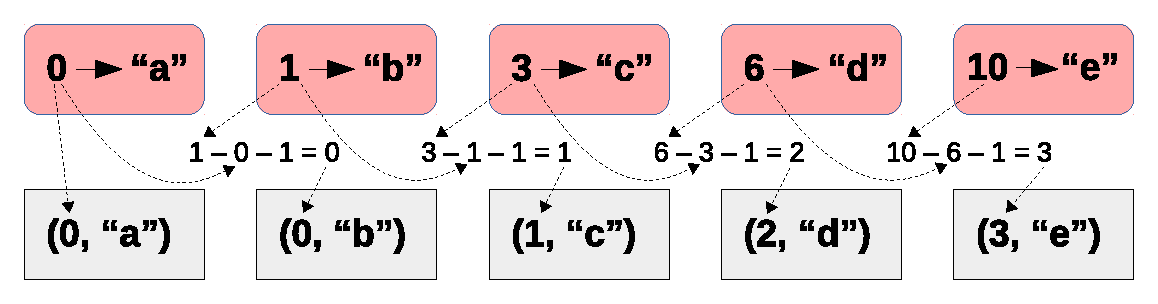
\includegraphics{figs/mech-1.eps}};
  \end{tikzpicture}
  \caption{How do we represent the mapping $\mapP$ as a \dd?}
  \label{fig:mech1}
\end{figure}
\begin{figure}[H]
  \centering
  \begin{tikzpicture}[nodes = {align = left}]
    \node [scale=.45]
    {\includegraphics{figs/find-6.eps}};
  \end{tikzpicture}
  \caption{How do we find key $6$ in the \dd?}
  \label{fig:find-6}
\end{figure}

TODO

\subsection{Metatheory}
\label{sec:Metatheory}
TODO

%\section{Evaluation}
%\label{sec:Evaluation}
% TODO delete? or keep?

\section{Discussion and Related Work}
\label{sec:Discussion}

Due to their simplicity, {\SAL}s are perhaps the most typical implementation for dictionaries.
%
However, \SemInj{} is of such importance in simplifying proofs that {\FPF}s, despite requiring a bit of extra overhead, also see significant use,
%
including in key works such as \emph{Software Foundations} \cite[Maps]{Pierce:SF1}.
%
{\CAL}s seem to get little use, perhaps because working with refinement proofs might add more hassle than \SemInj{} alleviates.
%
{\CAL}s are defined in the Coq standard library as \texttt{FMapList} \citep{XXX,XXX,XXX}; a Github search for \texttt{FMapList} shows $304$ results,
%
whereas a search for \texttt{FMapAVL} shows $474$ results, suggesting that {\CAL}s have been found to be less useful than high-performance implementations.
%
A search for \texttt{FunctionalExtensionality}, on the other hand, turns up $4916$ results, though most of these are probably unrelated to dictionaries.
%
\citep{XXX,XXX,XXX} \nick{Amorim ref} provides a more comprehensive treatment of {\CAL}s, augmenting them with a functional interface so that the client can
%
use them as though they were {\FPF}s.

% github searches
% funext        : 4916
% FMapInterface : 504
% FMapAVL       : 474
% FMapList      : 304

Sometimes, dictionaries are not used at all. When the order of bindings doesn't matter, dictionaries are a natural choice for type contexts,
%
but if types defined "later", or in inner scopes, can refer to to types defined in earlier/outer scopes, then order-insensitive dictionaries
%
are inherently inappropriate. This is the case with languages that support subtyping, notably the subject of the POPLMark challenge. Linear logics, on the other hand,
%
require sensitivity to duplicate insertions, so duplication-insensitive dictionaries are inappropriate for them as well. In these cases, {\SAL}s remain the most
%
natural choice, though future work could explore the possibility of data structures that are sensitive to ordering but not duplication, or vice versa.
%
Dictionary use is also avoided in many systems that use substitution rather than environments. For these reasons, many existing mechanizations make little use of
%
order-and-duplication-insensitive dictionaries. However, as mechanization becomes increasingly popular, for an ever-broadening scope of applications,
%
it seems inevitable that a programming utility as fundamental as dictionaries will eventually become ubiquitous, at which point it will be important to have the
%
best implementations at our disposal.


It was noted above that AVL implementations are apparently more popular than {\CAL}s, and as more software is mechanized, performance is likely to become an
%
even greater concern than it is today. In cases where there is no extraction step, and the proof language is also the language that will be executed,
%
there may be no choice but to use implementations that are high-performance but theoretically unwieldy. However, it seems more appropriate, especially with
%
fundamental utilities such as dictionaries, to either extract or transpile the mechanization into an implementation language that defines these utilities natively
%
by way of highly efficient implementations such as hashtables or red-black trees. This extraction may not be completely fidelitous, since it will be using a
%
different data structure in the implementation than was used in the proofs, but presumably the implementation's version of dictionaries is well-tested and bug-free,
%
and its definition of equality is, at least for fundamental utilities such as dictionaries, extensional and decidable. Regardless, even if unperformant implementations
%
cannot be used for code that will be run, they may be useful for parts of the code which are only used for proofs and will not be executed.


This paper discusses the important properties \SemTot, \SemInj, \EqDec, and \EzDstr, and offers an implementation for dictionaries that (mostly) fulfills these properties.
%
Future work could consider implementations for other key utilities, such as trees or graphs, that satisfy these properties. Doing so could be highly valuable,
%
but also far more challenging. It is relatively easy to simultaneously satisfy \SemTot{} and \SemInj{} for list-like structures such as dictionaries,
%
but much more awkward to do so for highly structural data such as graphs. For graphs in particular, establishing a one-to-one correspondence between terms and
%
semantic meanings requires understanding of the graph isomorphism problem, which besides being NP-hard, involves complex algebra.



\bibliography{references}

\end{document}
